\documentclass[handout, aspectratio=169]{beamer}
\mode<presentation>{}
\usepackage[utf8]{inputenc}
\newcommand{\fl}[1]{\left\lfloor #1 \right\rfloor}

\usepackage{tikz}

\title{MA 105 : Calculus\\ D1 - T5, Tutorial 04}  % change
\author{Aryaman Maithani}
\date[21-08-2019]{21st August, 2019}               % change
\institute[IITB]{IIT Bombay}
\usetheme{Warsaw}
\usecolortheme{beetle}
\newtheorem{defn}{Definition}
\begin{document}
\begin{frame}
	\titlepage
\end{frame}
\begin{frame}{Summary} 
	Sheet 3: Problems 4, 8 to 10\\	
	Sheet 4: Problems 2 to 4
\end{frame}
\begin{frame}{Sheet 3}                            % change
	4. (i) $p \le 0$ follows from question 2 of sheet 3. (Contrapositive)\\
	If $p = 0,$ then $f(x) = (x + q^{1/3})(x^2 - q^{1/3}x + q^{2/3}).$ The latter has no real roots if $q \neq 0.$ In the case that $q = 0,$ we still have only one (distinct) root.\\
	Thus, $p < 0.$ \hfill $\blacksquare$ \\~\\
	(ii) Let us look at $f'(x).$ \\
	We have it that $f'(x) = 3x^2 + p.$\\
	As $p < 0,$ we have it that $f'(x)$ has two distinct roots which are $x = \pm \sqrt{-p/3}.$\\
	By the second derivative test, it can be verified that we have maximum and minimum at $-\sqrt{-p/3}$ and $\sqrt{-p/3},$ respectively. \hfill $\blacksquare$ \\~\\
\end{frame}
\begin{frame}{Sheet 3}
	(iii) Let $\lambda := \sqrt{-p/3}.$ We have to show that $f(\lambda)$ and $f(-\lambda)$ are of different signs.\\
	We are given that $f(x)$ has three distinct roots. Let these roots be $\alpha, \beta, \gamma$ such that $\alpha < \beta < \gamma.$\\
	By Rolle's Theorem, we know that $f'(x)$ has a root in $(\alpha, \beta)$ and one in $(\beta, \gamma).$ Recall that we have already found all the roots of $f'(x).$ It must be the case that $\alpha < -\lambda < \beta < \lambda < \gamma.$\\
	Moreover, by looking at the sign of $f'(x),$ we know that $f$ is strictly decreasing in $[-\lambda, \lambda].$\\
	As we have it that $\beta \in [-\lambda, \lambda]$ and $f(\beta) = 0,$ we know that that $f(\lambda) < 0$ and $f(-\lambda) > 0.$ \hfill $\blacksquare$\\~\\
	%
	Thus, we now know that $f(\lambda)f(-\lambda) < 0.$
\end{frame}

\begin{frame}{Sheet 3}		
	\begin{align*}
	 	f(\lambda)f(-\lambda) &< 0\\
	 	(\lambda^3 + p\lambda + q)(-\lambda^3 - p\lambda + q) &< 0\\
	 	\implies q^2 - (\lambda^3 + p\lambda)^2 &< 0\\
	 	\implies q^2 - \lambda^2(\lambda^2 +p)^2 &< 0\\
	 	\implies q^2 + (p/3)(-p/3 + p)^2 &< 0\\
	 	\implies q^2 + 4p^3/27 &< 0\\
	 	\implies 4p^3 + 27q^2 &< 0 & \blacksquare
	\end{align*} 
\end{frame}
\begin{frame}{Sheet 3}
	8. (i) Not possible.\\
	Assume not. Then, we are given that $f''$ exists. Thus, $f'$ must be continuous and differentiable everywhere.\\
	We have that $f'(0) = f'(1).$ Thus, by Rolle's Theorem, $f''(c) = 0$ for some $c \in (0, 1).$ This contradicts the hypothesis. \hfill $\blacksquare$\\~\\
	(ii) Possible. $f: \mathbb{R} \to \mathbb{R}$ with $f(x) := x + \dfrac{x^2}{2}$ is one such function. \\~\\
	(iv) Possible. $f:\mathbb{R} \to \mathbb{R}$ with
	\[f(x) := \left\{\begin{array}{l r}
		\dfrac{1}{1- x} & \text{if } x \le 0\\
		1 + x + x^2	& \text{if } x > 0
	\end{array}
	\right.\]
	is one such function.
\end{frame}
	
\begin{frame}{Sheet 3}
	(iii) Not possible.\\
	Assume not. Then, we are given that $f''$ exists. Thus, $f'$ must be continuous and differentiable everywhere.\\
	As $f''$ is nonnegative, $f'$ must be increasing everywhere. We are given that $f'(0) = 1.$ \\
	Thus, given any $c > 0,$ we know that $f'(c) \ge 1.$ \hfill (1)\\
	Let $x \in (0, \infty).$ By MVT, we know that there exists $c \in (0, x)$ such that $f'(c) = \dfrac{f(x) - f(0)}{x - 0}.$ \\ Thus, by (1), we have it that $f(x) - f(0) \ge x$ for all positive $x.$ \\
	This contradicts that $f(x) \le 100$ for all positive $x.$ (How?)
\end{frame}

\begin{frame}{Sheet 3}
	9. As $f:[-2, 5] \to \mathbb{R}$ is continuous, we have it that the absolute extrema of $f$ on $[a, b]$ is attained either at a critical point of $f$ or at an end-point of $[a, b].$\\
	Recall that an interior point $c$ of the domain is called a critical point of $f$ if either $f$ is not differentiable at $c,$ or if $f$ is differentiable at $c$ and $f'(c) = 0.$\\
	It is clear that $0$ is a critical point as $f$ is not differentiable at $0.$ Moreover, $0$ is the only point at which $f$ is not differentiable.\\
	Rewriting $f(x),$ we get
	\[f(x) = \left\{\begin{array}{l r}
		1 - 12x - 3x^2  & \text{if } x \le 0\\
		1 + 12x - 3x^2	& \text{if } x > 0
	\end{array}
	\right.\]
	For $x < 0,$ we get the derivative of $f$ as $f'(x) = -12 - 6x = -6(x + 2).$ Thus, no negative number in the domain is a critical point. (Note that $-2$ is \textbf{not} an interior point of the domain.)
\end{frame}
\begin{frame}{Sheet 3}
	For $x > 0,$ we get the derivative as $f'(x) = 12 - 6x = 6(2 - x).$ Thus, $2$ is a critical point of $f.$ (Note that $2$ \textbf{is} an interior point of the domain.)\\~\\
	To summarise,\\
	Critical points of $f:$ $0, 2.$ End-points of $[-2, 5]:$ $-2, 5.$\\
	\begin{center}
		\begin{tabular}{|c| c c c c|}
		\hline
		x & 0 & 2 & -2 & 5\\
		f(x) & 1 & 13 & 13 & -14 \\
		\hline
		\end{tabular}
	\end{center}
	$\therefore f$ attains its global maximum $13$ at $2$ as well as $-2,$ and its global minimum $-14$ at $5.$
\end{frame}
\begin{frame}{Sheet 3}
	10.
	\begin{figure}
		\centering
		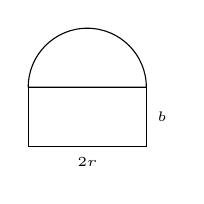
\begin{tikzpicture}
			\def \r{0.75}
			\def \b{0.75}
			\draw[] (0, \b) -- (0, 0) -- (2*\r, 0) -- (2*\r, \b);
			\draw[] (0, \b) -- (2*\r, \b) arc(0:180:\r);
			\node[] at (\r, - 0.2) {\tiny $2r$}; 
			\node[] at (2*\r + 0.2, \b/2) {\tiny $b$}; 
		\end{tikzpicture}
	\end{figure}
	%
	Let $l(r, b)$ denote the amount of light that enters through the window for $r$ and $b$ specified in the diagram.\\
	We know that $l(r, b) = k(2rb) + \left(\frac{k}{2}\right)(\frac{\pi r^2}{2}).$ Where $k$ is some positive constant.\\
	
	We are given that $p = 2b + 2r + \pi r = 2b + (2 + \pi)r$ is fixed. Thus, we can rewrite the amount of light just in terms of the radius as follows:\\
	$L(r) = l\bigg(r, \frac{1}{2}\big(p - (2 + \pi)r\big)\bigg) = k\left[r(p - (2 + \pi)r) + \frac{\pi r^2}{4}\right] = k \left[pr - 2r^2 - \frac{3\pi r^2}{4}\right].$\\
	As the above is defined for $(0, \infty)$ and is differentiable everywhere, we only need to check where the derivative is zero.\\~\\
\end{frame}
\begin{frame}{Sheet 3}
	$L'(r) = k\left[p - 4r - \frac{3\pi r}{2}\right] = k\left[p - \left(\frac{8 + 3\pi}{2}\right)r\right] .$\\
	$\therefore L'(r) = 0 \implies r = \dfrac{2p}{8 + 3\pi}.$\\~\\
	It can be easily verified that for this value of $r,$ $L''(r)$ is indeed negative. (In fact, it is always negative.)\\~\\
	$b$ can now be calculated as we know the relation between $b, p$ and $r.$\\
	It comes out to be $\dfrac{1}{2}\left(\dfrac{4 + \pi}{8 + 3\pi}\right)p.$
\end{frame}

\begin{frame}{Sheet 4}
	2. 
	\begin{figure}
		\centering
		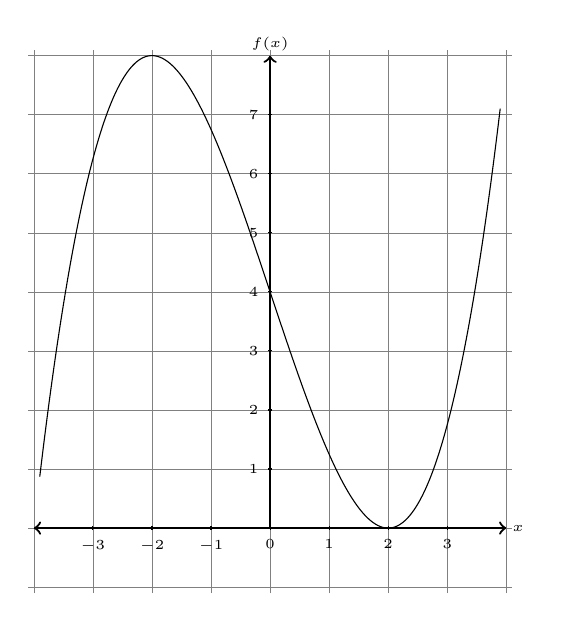
\begin{tikzpicture}[scale = 0.75]
			\draw[step=1cm,gray,very thin] (-4.1,-1.1) grid (4.1,8.1);
			\draw[thick,->] (0,0) -- (4,0);
			\draw[thick,->] (0,0) -- (0, 8);
			\draw[thick,->] (0,0) -- (-4,0);
			\node[] at (4.2, 0) {\tiny $x$};
			\node[] at (0, 8.2) {\tiny $f(x)$};
			\foreach \x in {-3, ..., 3}
   \draw (\x cm,1pt) -- (\x cm,-1pt) node[anchor=north] {\tiny $\x$};
\foreach \y in {1, ...,7}
    \draw (1pt,\y cm) -- (-1pt,\y cm) node[anchor=east] {\tiny $\y$};

    \draw[variable=\t,domain=-3.9:3.9,samples=500] plot ({\t},{0.25*\t*\t*\t - 3*\t + 4});

		\end{tikzpicture}
	\end{figure}
\end{frame}
\begin{frame}{Sheet 4}
	2. (contd.)\\
	I have actually graphed a polynomial that satisfies the given properties.\\
	Can you come up with it?\\
	Is there a unique such polynomial?\\
	What's the minimum degree of such a polynomial?\\
	Is there a unique polynomial with that degree?\\
	Suppose you have two distinct polynomials $f$ and $g$ that satisfy the given conditions. Can you come up with a distinct third polynomial such that it satisfies the conditions as well?
\end{frame}

\begin{frame}{Sheet 4}
	3. (i) $f(x) = x^2.$ \\
	 (ii) $f(x) = \sqrt{x}.$ \\
	 (iii) $f(x) = -\sqrt{x}.$ \\
	 (iv) $f(x) = -x^2.$ \\~\\
	 %
	 Note that these functions are strictly convex (or concave) as well.

\end{frame}
\begin{frame}{Sheet 4}
	4. (i) True.\\
	Note that we \textbf{cannot} use the derivative test to prove this as we do not know whether $f$ and/or $g$ are differentiable. (They may not even be continuous!)\\~\\
	%
	By definition, we know that there exists $\delta_1 > 0$ such that $f(c) \ge f(x)$ whenever $x \in (c - \delta_1, c + \delta_1).$\\
	Similarly, $\exists \delta_2 > 0$ such that $|x - c| < \delta_2 \implies g(x) \le g(c).$\\
	(Note how the same statement can be written in different styles.)\\
	Let $\delta := \min\{\delta_1, \delta_2\}.$ Thus, for $x \in (c-\delta, c+\delta),$ we know that $f(x) \le f(c)$ \emph{and} $g(x) \le g(c).$\\
	As $f(x)$ and $g(x)$ are always nonnegative, we know that
	\[h(c) = f(c)g(c) \ge f(c)g(x) \ge f(x)g(x) = h(x) \quad \forall x \in (c-\delta, c+\delta).\]
	Thus, $h$ has a local maximum at $c.$ \hfill $\blacksquare$
\end{frame}
\begin{frame}{Sheet 4}
	4. (ii) False.\\
	Take $f(x) = g(x) = x^4 - x^3 + 1.$\\
	Both $f$ and $g$ have a point of inflection at $0.5$ but $h$ does not. ($h''(0.5)$ turns out to be $0.125$)\\~\\
	A ``simpler'' counterexample would have probably been $f(x) = g(x) = 1 + \sin x.$ The reason I avoid this is because I wouldn't consider $\sin$ to be a simple function!\\
	It is for a similar reason that I did not give $e^x$ as an example for Question 8 part (iv).\\~\\
	Here's an even weirder example which I claim is a counterexample -
	\[f(x) = g(x) = |x|, \quad c = 0\]
	How's that for simplicity?\\
	Can you argue that $0$ indeed is a point of inflection of $f$ and $g?$ Can one even be so bold as to claim that \emph{all} real numbers are points of inflection of $f$ and $g$ both?
\end{frame}
\end{document}